\documentclass[11pt]{amsart}
\usepackage[T1]{fontenc}
\usepackage{lmodern}
\usepackage[margin=1.1in]{geometry}
\usepackage{amssymb,amsmath,mathtools}
\usepackage{booktabs}
\usepackage[hidelinks,hypertexnames=false]{hyperref}
\usepackage{xcolor}
\usepackage{tikz}
\usetikzlibrary{arrows.meta,calc,positioning,decorations.pathreplacing}
% Okabe--Ito colors used by the figures
\definecolor{pA}{HTML}{0072B2}\definecolor{pB}{HTML}{E69F00}\definecolor{pC}{HTML}{009E73}\definecolor{pD}{HTML}{CC79A7}
\setlength{\emergencystretch}{1.5em}

\newtheorem{theorem}{Theorem}[section]
\newtheorem{proposition}[theorem]{Proposition}
\newtheorem{lemma}[theorem]{Lemma}
\theoremstyle{remark}
\newtheorem{remark}[theorem]{Remark}

\newcommand{\F}{\mathbb{F}}
\newcommand{\Z}{\mathbb{Z}}
\newcommand{\R}{\mathbb{R}}
\DeclareMathOperator{\srg}{srg}
\DeclareMathOperator{\Aut}{Aut}

\title[Strongly regular graphs on 496 vertices]{Strongly regular graphs with parameters $(496,231,102,112)$}
\author{Dylan Plummer}
\date{25 November 2026}

\begin{document}

\begin{abstract}
Brouwer's table lists the parameters $(496,231,102,112)$ as open. We construct more than $7\cdot10^{107}$ pairwise non-isomorphic strongly regular graphs with these parameters. One starter under $\Z_7\times\F_2^2$ decomposes the complete multipartite graph $K_{15\times4}$ into $28$ copies of the triangular graph $T(6)$, and adding one point gives a Steiner system $S(2,5,61)$. Every point is replaced by $\F_2^3$, the seven tiles at a point receive the seven nonzero characters, and each tile is signed by the roots of $A_5$. This gives a regular two-graph on $496$ points, and switching by a $\pm1$ eigenvector of its Seidel matrix gives the graph. The design and the labels can be recovered from the two-graph, which gives the count. The same two-graphs also give more than $7\cdot10^{107}$ graphs with each of the known parameters $(496,240,120,112)$ and $(495,238,109,119)$. Up to $1300$ vertices, the only other open rows reached by the construction need an $S(2,6,76)$ tiled by copies of $T(7)$. A companion note uses the same local rule to construct $\srg(400,168,68,72)$.
\end{abstract}

\maketitle

\section{Introduction}

A two-graph is given by a Seidel matrix $S$, a symmetric matrix with zero diagonal and entries $\pm1$ off the diagonal, up to switching $S\mapsto DSD$ by diagonal $\pm1$ matrices $D$~\cite{Sei76}. It is regular when $S$ has exactly two eigenvalues~\cite{Tay77}. If $S$ has eigenvalues $\rho_1>0>\rho_2$ and a $\pm1$ eigenvector $w$, then switching by $\operatorname{diag}(w)$ gives a Seidel matrix with constant row sums, and the pairs with entry $-1$ form a strongly regular graph. We obtain the graphs this way.

Section~\ref{sec:tiling} gives the tiling, Section~\ref{sec:frame} the two-graph and Section~\ref{sec:graph} the eigenvector. Section~\ref{sec:count} proves the lower bound, Section~\ref{sec:symmetric} describes the members with the largest automorphism groups, Section~\ref{sec:known} compares the two-graphs with known ones, and Section~\ref{sec:other} lists the other parameters reached by the template. Figure~\ref{fig:flow} shows which results rest on computations.

The construction uses the same local rule as our construction of $\srg(400,168,68,72)$~\cite{P400}. There the complement of the Hoffman--Singleton graph is tiled by copies of $T(5)$ signed by the roots of $A_4$, every point is replaced by $\F_2^3$, and the seven tiles at a point receive the seven nonzero characters. Two vertices over points $p,q$ of a common tile are joined according to the product of their character values and the sign of the inner product of the two roots. Here the tiles are copies of $T(6)$ with the roots of $A_5$. The base graph $K_{15\times4}$ does not have a suitable spectrum, so we work with a frame instead: one coordinate per part ties together the four fibers of the part, and a fiber of $16$ vectors at the added point makes the frame tight. The result is a two-graph, and a switching gives the graph. The two constructions lead to the same next target on $616$ vertices (Section~\ref{sec:other} and~\cite{P400}).

\section{The tiling}\label{sec:tiling}

Let $G=\Z_7\times\F_2^2$, and encode $(a,b)\in G$ as $4a+b$. Take two copies of $G$ (sheets $0$ and $1$) and one copy of $\F_2^2$ (sheet $2$), $60$ points in all. Each of the two long sheets is split into seven parts of size four by the first coordinate, and sheet $2$ is the fifteenth part. The group $G$ acts on all three sheets by translation, on sheet $2$ through its second coordinate.

The starter assigns a point (sheet, position) to every edge of $K_6$:
\begin{center}\small
\begin{tabular}{@{}l*{15}{c}@{}}
\toprule
edge & 01&02&03&04&05&12&13&14&15&23&24&25&34&35&45\\
sheet& 2&0&1&1&1&1&0&0&0&1&1&1&0&0&0\\
pos & 0&0&5&10&19&0&9&18&7&13&26&23&4&16&8\\
\bottomrule
\end{tabular}
\end{center}
Two points of the starter are joined when their edges share a symbol, which gives a copy of $T(6)$.

\begin{lemma}\label{lem:tiling}
The $28$ translates of the starter are edge-disjoint copies of $T(6)$ that cover every edge of $K_{15\times4}$ exactly once, and every point lies in seven of them. Add a point $\infty$ to every part, and take for each tile and each symbol $u$ the five points whose edges contain $u$. The resulting $15+28\cdot6=183$ blocks form a Steiner system $S(2,5,61)$.
\end{lemma}

\begin{proof}
This is a difference computation. Within a long sheet, the twelve same-sheet differences of the starter, taken up to sign, are $4,\dots,15$, each once, and these are exactly the differences between points of different parts. Between sheets $0$ and $1$ all $28$ differences occur once. From each long sheet to the short one all four binary differences occur once, and a tile contains only one short-sheet point. No edge of the starter is fixed by a nontrivial translation, so the $60$ edges give $28\cdot60=1680$ edges, the number of edges of $K_{15\times4}$. A point has $56$ neighbors and each tile through it supplies eight, so it lies in seven tiles. Two blocks from the same tile meet in the point of their common edge. Two points in different parts lie in exactly one common tile and share exactly one symbol there, and two points in the same part lie in the part block. So every pair of the $61$ points is in exactly one block.
\end{proof}

A tile can contain two points of the same part (each tile meets only $12$ of the $15$ parts), but such points are never adjacent in the tile.

\begin{remark}\label{rem:starters}
A companion search enumerated the starters of this shape that are also invariant under an element of order three, which acts as the cycle $(3\,4\,5)$ on the symbols and as a multiplier on $G$. It found $216$ starters, whose designs fall into three isomorphism classes of $72$ each. One class is the design above. Representatives of the other two agree with the table above on the edges $01,\dots,05,12$ and on all sheets, and have the following positions on the other nine edges:
\begin{center}\small
\begin{tabular}{@{}l*{9}{c}@{}}
\toprule
edge & 13&14&15&23&24&25&34&35&45\\
\midrule
design 01 & 10&19&5&13&26&23&6&17&11\\
design 02 & 19&5&10&17&6&11&13&23&26\\
\bottomrule
\end{tabular}
\end{center}
We checked independently that both starters satisfy Lemma~\ref{lem:tiling}, that the three designs are pairwise non-isomorphic, and that each has an automorphism group of order $84$ fixing $\infty$. Everything below applies to all three designs. The search did not cover starters without the extra symmetry.
\end{remark}

\section{The two-graph}\label{sec:frame}

For $c,x\in\F_2^m$ write $\chi_c(x)=(-1)^{c\cdot x}$. The construction uses the following labels.
\begin{itemize}
\item At each of the $60$ points $p$: a bijection $c_p$ from the seven tiles through $p$ to the nonzero vectors of $\F_2^3$, and a sign $\varepsilon_p(T)$ for each such tile $T$.
\item At $\infty$: a bijection $g\mapsto u_g$ from the $15$ parts to the nonzero vectors of $\F_2^4$.
\end{itemize}
The matrix $F$ has one row for each part and six rows for each tile, one per symbol, so $15+28\cdot6=183$ rows. Its columns are the following (Figure~\ref{fig:frame}).
\begin{itemize}
\item Sixteen columns at $\infty$, one for each $x\in\F_2^4$, with entry $\chi_{u_g}(x)$ in the row of part $g$ and zero elsewhere.
\item Eight columns at each point $p$, one for each $x\in\F_2^3$. The column has a $1$ in the row of the part of $p$. In each tile $T$ through $p$, where $p$ is the edge $ab$ with $a<b$, it has $\varepsilon_p(T)\chi_{c_p(T)}(x)$ in row $a$ and $-\varepsilon_p(T)\chi_{c_p(T)}(x)$ in row $b$.
\end{itemize}
So the tile part of a column at $p$ is $\pm(e_a-e_b)$, a root of $A_5$. We call the $16$ columns at $\infty$ and the eight columns at each point the \emph{cells}.

\begin{figure}[t]
\centering
\resizebox{\textwidth}{!}{% Figure 1: (a) the shape of the 183 x 496 matrix F, (b) one tile block of one point, entry by entry.
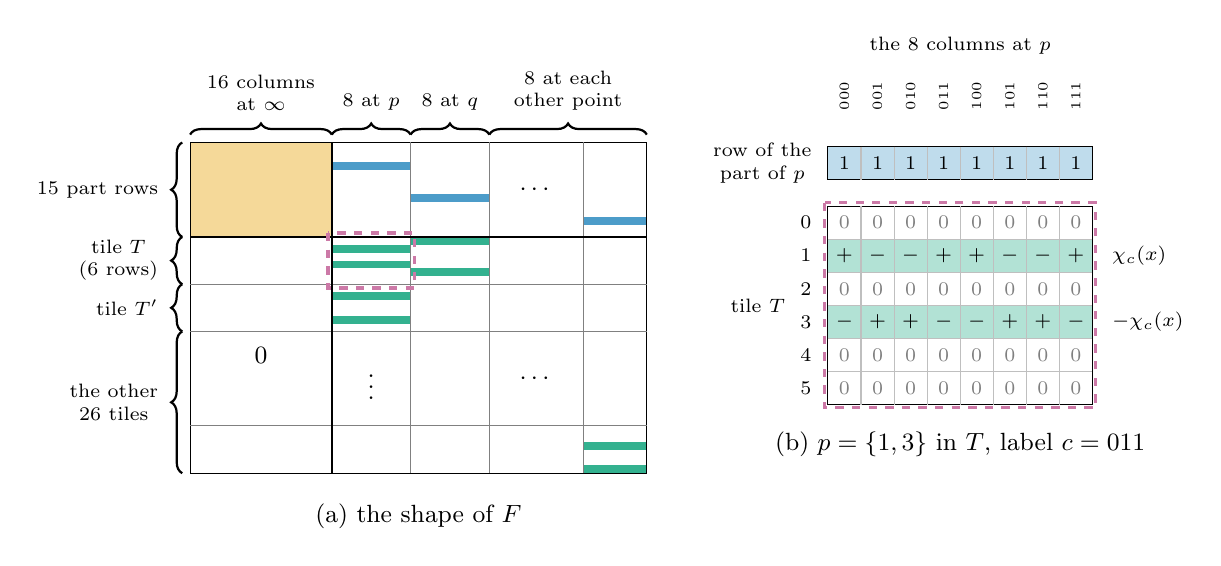
\begin{tikzpicture}[font=\small, x=1cm, y=1cm,
  brace/.style={decorate, decoration={brace, amplitude=4pt}, thick},
  lab/.style={font=\scriptsize, align=center},
  pm/.style={font=\scriptsize}]
% ================= (a) shape of F =================
% columns: inf [0,1.8], p [1.8,2.8], q [2.8,3.8], dots [3.8,5.0], last point [5.0,5.8]
% rows: parts [0,-1.2]; tiles: T [-1.2,-1.8], T' [-1.8,-2.4], dots [-2.4,-3.6], last tile [-3.6,-4.2]
\fill[pB!40] (0,0) rectangle (1.8,-1.2);
% part rows: one row of ones per point
\fill[pA!70] (1.8,-0.25) rectangle (2.8,-0.35);
\fill[pA!70] (2.8,-0.65) rectangle (3.8,-0.75);
\fill[pA!70] (5.0,-0.95) rectangle (5.8,-1.05);
% tile T contains p and q; tile T' contains p only; the last tile contains the last point
\foreach \x/\w/\ya/\yb in {1.8/1.0/-1.3/-1.5, 2.8/1.0/-1.2/-1.6, 1.8/1.0/-1.9/-2.2, 5.0/0.8/-3.8/-4.1} {
  \fill[pC!80] (\x,\ya) rectangle ++(\w,-0.1);
  \fill[pC!80] (\x,\yb) rectangle ++(\w,-0.1);}
% grid
\draw (0,0) rectangle (5.8,-4.2);
\foreach \x in {2.8,3.8,5.0} \draw[gray] (\x,0) -- (\x,-4.2);
\foreach \y in {-1.8,-2.4,-3.6} \draw[gray] (0,\y) -- (5.8,\y);
\draw[thick] (0,-1.2) -- (5.8,-1.2);
\draw[thick] (1.8,0) -- (1.8,-4.2);
\node at (4.4,-0.6) {$\cdots$}; \node at (4.4,-3.0) {$\cdots$}; \node at (2.3,-3.0) {$\vdots$}; \node at (0.9,-2.7) {$0$};
% zoom marker
\draw[pD, very thick, dashed] (1.75,-1.15) rectangle (2.85,-1.85);
% column braces
\draw[brace] (0,0.1) -- node[lab, above=5pt] {$16$ columns\\ at $\infty$} (1.8,0.1);
\draw[brace] (1.8,0.1) -- node[lab, above=5pt] {$8$ at $p$} (2.8,0.1);
\draw[brace] (2.8,0.1) -- node[lab, above=5pt] {$8$ at $q$} (3.8,0.1);
\draw[brace] (3.8,0.1) -- node[lab, above=5pt] {$8$ at each\\ other point} (5.8,0.1);
% row braces
\draw[brace] (-0.1,-1.2) -- node[lab, left=5pt] {$15$ part rows} (-0.1,0);
\draw[brace] (-0.1,-1.8) -- node[lab, left=5pt] {tile $T$\\ ($6$ rows)} (-0.1,-1.2);
\draw[brace] (-0.1,-2.4) -- node[lab, left=5pt] {tile $T'$} (-0.1,-1.8);
\draw[brace] (-0.1,-4.2) -- node[lab, left=5pt] {the other\\ $26$ tiles} (-0.1,-2.4);
\node at (2.9,-4.75) {(a) the shape of $F$};
% ================= (b) zoom: point p in tile T =================
\begin{scope}[xshift=8.1cm, yshift=0.2cm, x=0.42cm, y=0.42cm]
  % columns x = 000..111, chi_c(x) for c = 011: + - - + + - - +
  \foreach \k/\b in {0/000,1/001,2/010,3/011,4/100,5/101,6/110,7/111}
    \node[font=\tiny, rotate=90, anchor=west] at (\k+0.5,0.2) {\b};
  \node[lab, anchor=south] at (4,1.9) {the $8$ columns at $p$};
  % part row of p
  \foreach \k in {0,...,7} {\fill[pA!25] (\k,-0.6) rectangle ++(1,-1); \node[pm] at (\k+0.5,-1.1) {$1$};}
  \draw (0,-0.6) rectangle (8,-1.6);
  \node[lab, anchor=east] at (-0.2,-1.1) {row of the\\ part of $p$};
  % tile block rows 0..5, starting at y=-2.4
  \foreach \r in {0,...,5} \node[pm, anchor=east] at (-0.2,-2.9-\r) {\r};
  \node[lab, anchor=east] at (-1.0,-5.4) {tile $T$};
  \foreach \k/\s/\t in {0/+/-,1/-/+,2/-/+,3/+/-,4/+/-,5/-/+,6/-/+,7/+/-} {
    \fill[pC!30] (\k,-3.4) rectangle ++(1,-1);
    \node[pm] at (\k+0.5,-3.9) {$\s$};
    \fill[pC!30] (\k,-5.4) rectangle ++(1,-1);
    \node[pm] at (\k+0.5,-5.9) {$\t$};}
  \foreach \r in {0,2,4,5} \foreach \k in {0,...,7} \node[pm, gray] at (\k+0.5,-2.9-\r) {$0$};
  \draw (0,-2.4) rectangle (8,-8.4);
  \foreach \y in {-3.4,-4.4,-5.4,-6.4,-7.4} \draw[gray!50] (0,\y) -- (8,\y);
  \foreach \x in {1,...,7} \draw[gray!50] (\x,-0.6) -- (\x,-1.6) (\x,-2.4) -- (\x,-8.4);
  \node[lab, anchor=west] at (8.3,-3.9) {$\chi_c(x)$};
  \node[lab, anchor=west] at (8.3,-5.9) {$-\chi_c(x)$};
  \draw[pD, very thick, dashed] (-0.1,-2.3) rectangle (8.1,-8.5);
  \node at (4,-9.6) {(b) $p=\{1,3\}$ in $T$, label $c=011$};
\end{scope}
\end{tikzpicture}
}
\caption{(a) The shape of $F$. Colored entries are $\pm1$ and blank entries are $0$. The $16$ columns at $\infty$ are nonzero only in the part rows, where they form a Walsh--Hadamard block. The $8$ columns at a point $p$ have a row of ones in the row of the part of $p$ (blue) and two nonzero rows in each of the seven tiles through $p$ (green); $T$ and $T'$ are two of these tiles, and $T$ also contains $q$. (b) The dashed block of (a) in detail, for $p$ the edge $\{1,3\}$ of $T$ with label $c=011$ and sign $+1$. Rows $1$ and $3$ carry $\chi_c(x)$ and $-\chi_c(x)$, so the part of each column in $T$ is $\pm(e_1-e_3)$.}
\label{fig:frame}
\end{figure}

\begin{proposition}\label{prop:frame}
For all labels and signs, every column of $F$ has squared norm $15$, two distinct columns have inner product $\pm1$, and $FF^{\top}$ is $48$ times an orthogonal projection of rank $155$. Hence $S=F^{\top}F-15I$ is the Seidel matrix of a regular two-graph $\Omega$ on $496$ points, with eigenvalues $33$ (multiplicity $155$) and $-15$ (multiplicity $341$).
\end{proposition}

\begin{proof}
A column at a point has squared norm $1+7\cdot2=15$, and a column at $\infty$ has squared norm $15$. Two columns $x\ne y$ at one point have inner product $1+2\sum_{c\ne0}\chi_c(x+y)=1-2=-1$, and two columns at $\infty$ have $\sum_{u\ne0}\chi_u(x+y)=-1$. Columns at two points of one part meet only in the part row. Two points in different parts are adjacent in exactly one tile, where their roots have inner product $\pm1$, and they share no other row. A column at $\infty$ and a column at a point meet only in one part row.

By orthogonality of characters, the rows of $F$ are pairwise orthogonal, except for the six rows of a tile. A part row has squared norm $16+4\cdot8=48$. On the six rows of a tile, $FF^{\top}$ equals $8\sum_{ab}(e_a-e_b)(e_a-e_b)^{\top}=8(6I-J)$, which is $48$ times the projection onto the complement of the all-ones vector. So $FF^{\top}$ is $48$ times a projection of rank $15+28\cdot5=155$, and $F^{\top}F$ has eigenvalues $48$ and $0$ with multiplicities $155$ and $341$.
\end{proof}

\begin{proposition}[computational]\label{prop:steinerhalf}
At a point $p$, label the part block by $(0,0,0,1)\in\F_2^4$ and, in a tile where $p$ is the edge $ab$ with label $c$, label the stars of $a$ and $b$ by $(c,0)$ and $(c,1)$, in an order fixed by $\varepsilon_p(T)$. At $\infty$, label part $g$ by $u_g$. The Steiner equiangular tight frame~\cite{FMT12} of the $S(2,5,61)$ with these labels has $61\cdot16=976$ columns in $\R^{183}$ and Seidel eigenvalues $65$ and $-15$. Up to sign, the $496$ columns of $F$ are its $16$ columns at $\infty$ and, at each point, the $8$ columns whose last coordinate is $1$.
\end{proposition}

So $\Omega$ is a regular sub-two-graph of the Steiner two-graph of the $S(2,5,61)$.

\section{The graph}\label{sec:graph}

Mark the symbols $0$ and $1$ of $K_6$ (Figure~\ref{fig:tile}). An edge \emph{crosses} if it joins a marked symbol to an unmarked one. The edge $01$ of the starter lies on the short sheet, and the eight crossing edges have four positions on each long sheet. By translation, every point of a long sheet is a crossing edge in four of its seven tiles, and a point of the short sheet in none. We call these four tiles the crossing tiles at $p$ and the other three the quiet tiles.

\begin{figure}[t]
\centering
% Figure 1: (a) one tile, (b) the labels at a long-sheet point.
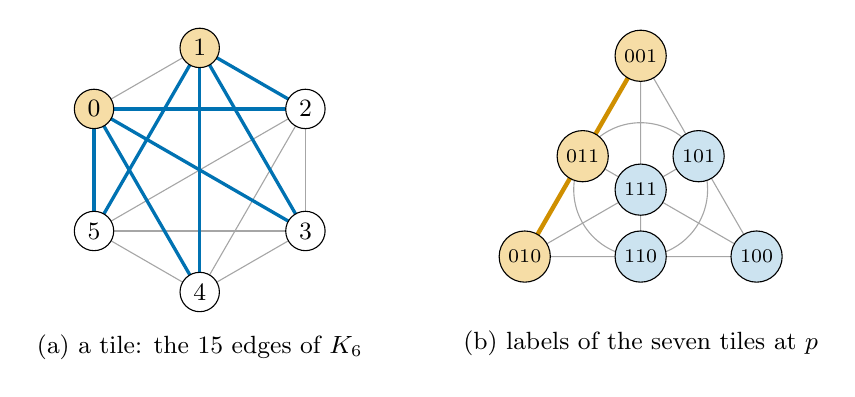
\begin{tikzpicture}[font=\small,
  sym/.style={circle, draw, inner sep=1.5pt, minimum size=5mm, fill=white},
  mk/.style={sym, fill=pB!35},
  cross/.style={pA, very thick},
  quiet/.style={gray!70, thin},
  fp/.style={circle, draw, inner sep=1pt, minimum size=6.5mm, font=\scriptsize, fill=white},
  fq/.style={fp, fill=pB!35},
  fc/.style={fp, fill=pA!20}]
% ---- (a) K6 with the cut {0,1} | {2,3,4,5}
\begin{scope}
  \foreach \i/\ang in {0/150,1/90,2/30,3/-30,4/-90,5/-150} \coordinate (s\i) at (\ang:1.55);
  \foreach \a/\b in {0/1,2/3,2/4,2/5,3/4,3/5,4/5} \draw[quiet] (s\a) -- (s\b);
  \foreach \a in {0,1} \foreach \b in {2,3,4,5} \draw[cross] (s\a) -- (s\b);
  \node[mk] at (s0) {0}; \node[mk] at (s1) {1};
  \foreach \i in {2,3,4,5} \node[sym] at (s\i) {\i};
  \node at (0,-2.25) {(a) a tile: the $15$ edges of $K_6$};
\end{scope}
% ---- (b) Fano plane of labels at a point on a long sheet
\begin{scope}[xshift=5.6cm, yshift=-0.25cm]
  \coordinate (A) at (90:1.7); \coordinate (B) at (210:1.7); \coordinate (C) at (330:1.7);
  \coordinate (AB) at ($(A)!0.5!(B)$); \coordinate (BC) at ($(B)!0.5!(C)$); \coordinate (CA) at ($(C)!0.5!(A)$);
  \coordinate (O) at (0,0);
  \draw[gray!70] (A) -- (BC) (B) -- (CA) (C) -- (AB) (B) -- (C) (C) -- (A);
  \draw[gray!70] (O) circle (0.85);
  \draw[pB!90!black, line width=1.6pt] (A) -- (B);
  \node[fq] at (A) {001}; \node[fq] at (B) {010}; \node[fq] at (AB) {011};
  \node[fc] at (C) {100}; \node[fc] at (BC) {110}; \node[fc] at (CA) {101}; \node[fc] at (O) {111};
  \node at (0,-1.95) {(b) labels of the seven tiles at $p$};
\end{scope}
\end{tikzpicture}

\caption{(a) A tile. Its points are the edges of $K_6$, joined when they share a symbol. The symbols $0,1$ are marked, and the eight crossing edges are blue. (b) The labels at a point $p$ of a long sheet are the points of the Fano plane. For admissible labels the three quiet tiles carry a line (orange), and the four crossing tiles carry the complement (blue), whose signs have product $-1$.}
\label{fig:tile}
\end{figure}

We call the labels \emph{admissible} if at every point of a long sheet the labels of the three quiet tiles, together with $0$, form a subspace of $\F_2^3$, and the signs of the four crossing tiles have product $-1$.

\begin{theorem}\label{thm:main}
Suppose the labels are admissible and $g_0$ is the short part. Let $z\in\R^{183}$ be $1$ in the row of $g_0$, $\tfrac12$ in the rows $0$ and $1$ of every tile, and $0$ elsewhere. Then $w=F^{\top}z$ is a $\pm1$ vector with $Sw=33w$. The pairs $i\ne j$ with $w_iS_{ij}w_j=-1$ form a strongly regular graph with parameters $(496,231,102,112)$. Its complement has parameters $(496,264,144,136)$.
\end{theorem}

\begin{proof}
At a column $x$ at $\infty$, $w=\chi_{u_{g_0}}(x)$. At a column at a short-sheet point, $w=1$. At a column $x$ at a long-sheet point only the four crossing tiles contribute, each $\pm\tfrac12\chi_c(x)$, because a crossing root $e_a-e_b$ has $a\in\{0,1\}$. So $w=\tfrac12\sum_{i=1}^4\eta_i\chi_{c_i}(x)$, where $c_1,\dots,c_4$ are the four labels outside a subspace, so that $c_4=c_1+c_2+c_3$, and $\eta_1\eta_2\eta_3\eta_4=-1$. Since $\chi_{c_4}=\chi_{c_1}\chi_{c_2}\chi_{c_3}$, checking the eight sign patterns of $(\chi_{c_1},\chi_{c_2},\chi_{c_3})$ gives $w=\pm1$. As $w$ lies in the image of $F^{\top}$, where $F^{\top}F$ acts as $48$, we get $Sw=33w$. Then $DSD$ with $D=\operatorname{diag}(w)$ has constant row sum $33$, so the graph is regular of degree $(495-33)/2=231$. Its other eigenvalues are $-(1+33)/2=-17$ and $-(1-15)/2=7$, so $A^2=119I-10A+112J$, which gives $\lambda=102$ and $\mu=112$.
\end{proof}

The exported graph uses, at a long-sheet point, the labels $4,5,6,7$ (as binary numbers) on the crossing tiles and $1,2,3$ on the quiet tiles, each in tile order, with sign $+1$ everywhere except on the crossing tile with label $7$. At a short-sheet point it uses $1,\dots,7$ in tile order with signs $+1$, and at $\infty$ part $g$ gets $u_g=g+1$. Its automorphism group, computed with nauty and with bliss, is $C_2\times C_2$.

\section{Counting the graphs}\label{sec:count}

The labels induce structures on the base that do not depend on the choice of coordinates. At a point $p$, the triples of tiles whose labels sum to zero are the lines of a Fano plane on the seven tiles at $p$. At $\infty$, the triples of parts whose labels sum to zero are the lines of a projective space $PG(3,2)$ on the $15$ parts. Admissibility says that the quiet tiles at each long-sheet point form a line.

\begin{lemma}[finite check]\label{lem:recovery}
Let $\Omega$ come from admissible labels on one of the three designs, let $S'$ be any Seidel matrix of $\Omega$, and put $M=S'-I$. The sets of four vertices whose rows of $M$ have a constant entrywise product are exactly the $140+60\cdot14=980$ affine planes inside the cells. Consequently $\Omega$ determines the cells, the parts, the tiles, the design, the Fano plane at every point and the $PG(3,2)$ on the parts.
\end{lemma}

\begin{proof}[Sketch]
The property does not change under switching or relabeling. Inside a cell every entry of $M$ is $-1$, and the restriction of a row to another cell is $\pm$ a character, so the affine planes have the property. To show that no other set does, consider the cells that the four vertices meet an odd number of times. On a further cell, the product of the four rows is a character determined by the tiles that join those cells to it, so it does not depend on the labels or signs. Running through all sets of at most four cells leaves only sets inside one part, and these fail on the cell at $\infty$ or on their own cells. For two pairs in two different cells, the supports of the row differences are distinct for all $2{,}100$ choices of a point and four tiles, and none is a union of parts. So the qualifying sets are the planes, and the cells are the connected components of the planes, with the cell at $\infty$ the one of size $16$.

On the cell at $\infty$, the rows of the vertices at a point are $\pm$ a common function times the character of their part. This recovers the parts, and removing the common function recovers the $PG(3,2)$. On the cell of a point, dividing by the row of a vertex at $\infty$ removes the switching, and the other parts show the characters of the tiles at that point. Triples of tiles whose characters multiply to a constant are the Fano lines. Joining the tiles that two points assign to each other gives the $28$ copies of $T(6)$, and their $5$-cliques are the stars.
\end{proof}

The finite checks of the first paragraph are made by \texttt{extensions/starters/recover.py}. Our script \texttt{extensions/designs\_audit.py} also applies random switchings and relabelings to random admissible members of all three designs, and finds exactly the $980$ planes each time.

\begin{theorem}\label{thm:count}
Admissible labels on the three designs give more than
\[
\frac{6^{56}\cdot30^{4}}{84}\cdot\frac{15!}{20160}\cdot2^{152}\bigl(2^{22}+2\cdot2^{19}\bigr)>7.06\cdot10^{107}
\]
pairwise non-isomorphic regular two-graphs. Each contains a strongly regular graph with parameters $(496,231,102,112)$ and one with parameters $(496,240,120,112)$, and each has descendants with parameters $(495,238,109,119)$. So each of these rows, and the complementary rows $(496,264,144,136)$ and $(496,255,126,136)$, has more than $7.06\cdot10^{107}$ pairwise non-isomorphic members.
\end{theorem}

\begin{proof}
On seven labeled tiles there are $7!/168=30$ Fano planes, and $6$ of them contain a given triple as a line. So the Fano planes allowed by admissibility give $6^{56}\cdot30^4$ choices, and the $PG(3,2)$ structures on the parts give $15!/20160$ choices. For each of these structures, fix one labeling that induces it. The signs give $2^6$ choices at each long-sheet point (three quiet signs and three free crossing signs) and $2^7$ at each short-sheet point, $2^{364}$ in all.

Fix a design, and suppose two such choices give isomorphic two-graphs. By Lemma~\ref{lem:recovery}, the isomorphism induces one of the $84$ automorphisms of the design, and this automorphism determines the second choice of structures from the first. On each cell the isomorphism preserves affine planes, so it is affine, and its linear part is fixed by the characters it has to carry. That leaves at most $16\cdot8^{60}=2^{184}$ vertex permutations. For fixed labels and a fixed permutation, two sign choices that give the same labeled two-graph give equal Seidel matrices: the matrices agree on the cell at $\infty$ and between it and every other vertex, so any switching between them is constant. On each edge of a tile this fixes the product of two signs, and since $T(6)$ is connected, the signs in a tile are determined up to reversing all of them. A set of tile reversals keeps the labels admissible only if it contains an even number of the crossing tiles at every long-sheet point. The $56\times28$ matrix of crossing tiles has rank $22$ over $\F_2$ for the first design and $19$ for the other two, which allows $2^6$, $2^9$ and $2^9$ reversals. So an isomorphism class contains at most $84\cdot2^{184}\cdot2^{28-r}$ choices, where $r$ is the rank. Dividing gives the three terms of the bound. Non-isomorphic designs give non-isomorphic two-graphs by Lemma~\ref{lem:recovery}.

For the second row, let $w$ be $1$ on the cell at $\infty$ and, in each part, $-1$ on the cells of two of its four points and $1$ on the other two. Then $Fw=0$. In a part row the columns at $\infty$ sum to zero and the four cells cancel, and in a tile row each cell contributes a full character sum, which is zero. So $Sw=-15w$, and the pairs with $w_iS_{ij}w_j=+1$ form a regular graph of degree $(495-15)/2=240$, which is strongly regular with parameters $(496,240,120,112)$. A descendant (switch one vertex to be isolated and delete it) is strongly regular with parameters $(495,238,109,119)$ because $S^2=18S+495I$, and it determines its two-graph. Isomorphic graphs in these rows come from isomorphic two-graphs, so each row inherits the bound.
\end{proof}

The rows $(496,240,120,112)$ and $(495,238,109,119)$ were known before (Brouwer's table lists constructions by Wallis and from $O^-(10,2)$, among others), so for them Theorem~\ref{thm:count} is only a count. Without the restriction on tile reversals, the bound is still above $4.03\cdot10^{101}$. The bound and the ranks were computed twice, by \texttt{extensions/starters/plane\_count.py} and by \texttt{extensions/designs\_audit.py}, which also enumerates the $30$ Fano planes. In a separate test, $50$ random choices on the first design gave $50$ pairwise non-isomorphic graphs, all with trivial automorphism group.

\section{Symmetric members}\label{sec:symmetric}

On the first design the labels can be chosen compatibly with the symmetry of the starter. Identify $\F_2^3$ with $\F_8=\F_2[\alpha]/(\alpha^3+\alpha+1)$ and use $\chi_c(x)=(-1)^{\operatorname{Tr}(cx)}$. At the origin of each long sheet, give the crossing tiles labels of trace $1$, and require that the order-three symmetry (doubling the $\Z_7$ coordinate and cycling the nonzero elements of $\F_2^2$) send a tile labeled $c$ to a tile labeled $c^2$. Then transport the labels by translation. There are nine such choices on each long sheet.

\begin{proposition}[computational]\label{prop:symmetric}
The $81$ choices give nine pairwise non-isomorphic two-graphs. Each has an automorphism group of order $84$, generated by the $28$ translations and an element of order three, which preserves the Seidel matrix $S$ itself and fixes the cell at $\infty$.
\begin{enumerate}
\item The descendants fall into $14$ classes for each two-graph, $126$ in all, with automorphism groups of orders $1,3,12,21,84$ (for $36,45,18,9,18$ of them).
\item The $\pm1$ eigenvectors for $33$ obtained from cuts as in Theorem~\ref{thm:main} give $56$ pairwise non-isomorphic graphs with parameters $(496,231,102,112)$, with automorphism groups of orders $2,12,14,84$ (for $9,18,11,18$ of them).
\item The $\pm1$ vectors in the kernel of $F$ that are constant on every cell at a point are the vectors used in the proof of Theorem~\ref{thm:count}, together with those that equal $\chi_{u_g}$ on the cell at $\infty$ and are $-1$ on three cells of part $g$ and on two cells of every other part. By Burnside's lemma over the group of order $84$, they give exactly $61{,}571{,}844{,}416$ classes of graphs with parameters $(496,240,120,112)$ for each two-graph, and $554{,}146{,}599{,}744$ in all.
\end{enumerate}
\end{proposition}

We checked the group orders independently. Nauty finds $84$ automorphisms of the graph formed by the entries $-1$ of $S$. Descendants at vertices in different orbits of this group are non-isomorphic, and for every orbit the orbit length times the order of the automorphism group of the descendant is $84$, so the two-graph has exactly $84$ automorphisms. The $126$ descendants are pairwise non-isomorphic, so the nine two-graphs are too. We recomputed the Burnside count from the group found by nauty, including the sign with which each element maps the characters at $\infty$, and every exported graph was checked on all pairs.

\section{Comparison with known two-graphs}\label{sec:known}

In~\cite{P442} we showed that no Steiner two-graph built from an $S(2,3,31)$ (on $496$ points) or from an $S(2,5,61)$ (on $976$ points) with a Hadamard matrix of order $16$ contains a regular graph of degree $231$ or $455$, respectively. By Proposition~\ref{prop:steinerhalf}, $\Omega$ is half of a Steiner two-graph on $976$ points, so this result does not apply to it. Since $\Omega$ contains a regular graph of degree $231$, it is not the Steiner two-graph of any $S(2,3,31)$. Regular graphs in Steiner two-graphs of designs with a parallel class were found in~\cite[Theorem~3.6]{FJMPW18}. Here the regular graph lies in a sub-two-graph instead.

\begin{proposition}[computational]\label{prop:notsymplectic}
No two-graph of Theorem~\ref{thm:count} is isomorphic to the symplectic regular two-graph on $496$ points or to its complement.
\end{proposition}

\begin{proof}
The symplectic two-graph, with Seidel matrix $(-1)^{B(a,b)}$ on the $496$ singular vectors of an elliptic quadric in $\F_2^{10}$, has eigenvalues $15$ and $-33$, and its complement has $33$ and $-15$. Both are $2$-transitive; nauty gives the descendant an automorphism group of order $5.00308\cdot10^{13}=|Sp(10,2)|/496$. By Lemma~\ref{lem:recovery}, every automorphism of one of our two-graphs fixes the cell of size $16$, so its automorphism group is not transitive. For the exported example we also computed descendant automorphism groups directly: order $4$ at the three vertices at $\infty$ tested and order $1$ at the five other vertices tested.
\end{proof}

The descendants of the exported example are graphs $\srg(495,238,109,119)$ with at most four automorphisms. We have not compared them with every known graph with these parameters.

\section{Other parameters}\label{sec:other}

The construction works for any decomposition of $K_{P\times(m-2)}$ into copies of $T(m)$, with $P$ odd and Hadamard matrices of orders $P+1$ and $(P+1)/2$. Every point lies in $(P-1)/2$ tiles, and adding a point gives an $S(2,m-1,1+P(m-2))$. The columns have squared norm $P$, the part rows have squared norm $(P+1)m/2$, and each tile contributes $\tfrac{P+1}2(mI-J)$. So the frame has
\[
N=\tfrac12(P+1)\bigl(P(m-2)+2\bigr)\ \text{vectors},\qquad\text{rank } P+t(m-1)\ \text{for } t \text{ tiles},
\]
and Seidel eigenvalues $(P+1)m/2-P$ and $-P$. Table~\ref{tab:template} lists the cases with $N\le1300$.

\begin{table}[ht]
\centering\small
\caption{The template up to $1300$ vertices (status from Brouwer's table, 24 November 2026).}
\label{tab:template}
\begin{tabular}{@{}rrlrrl@{}}
\toprule
$P$ & $m$ & design & $N$ & eigenvalues & regular members \\
\midrule
$3$ & $3$ & $S(2,2,4)$ & $10$ & $3,-3$ & $(10,3,0,1)$, $(10,6,3,4)$: known\\
$3$ & $4$ & $S(2,3,7)$ & $16$ & $5,-3$ & $(16,5,0,2)$, $(16,9,4,6)$: known\\
$7$ & $3$ & $S(2,2,8)$ & $36$ & $5,-7$ & known\\
$7$ & $4$ & $S(2,3,15)$ & $64$ & $9,-7$ & known\\
$7$ & $7$ & $S(2,6,36)$ & $148$ & $21,-7$ & design does not exist (affine plane of order $6$)\\
$15$ & $3$ & $S(2,2,16)$ & $136$ & $9,-15$ & known\\
$15$ & $4$ & $S(2,3,31)$ & $256$ & $17,-15$ & known\\
$15$ & $6$ & $S(2,5,61)$ & $496$ & $33,-15$ & $(496,231,102,112)$: \textbf{this note}; $(496,255,126,136)$: known\\
$15$ & $7$ & $S(2,6,76)$ & $616$ & $41,-15$ & $(616,287,126,140)$, $(616,315,154,168)$: open\\
$31$ & $3$ & $S(2,2,32)$ & $528$ & $17,-31$ & known\\
$31$ & $4$ & $S(2,3,63)$ & $1024$ & $33,-31$ & known\\
$39$ & $3$ & $S(2,2,40)$ & $820$ & $21,-39$ & known\\
\bottomrule
\end{tabular}
\end{table}

For $m=3$ the tiles are triangles and the data is a Steiner triple system on $P$ parts of size one. The only other open case is $P=15$, $m=7$. It needs $25$ copies of $T(7)$ decomposing $K_{15\times5}$, that is, an $S(2,6,76)$ with a point whose other $175$ blocks split into $25$ sets of seven pairwise intersecting blocks. The two-graph on $616$ points would have Seidel eigenvalues $41$ and $-15$, and its descendants would be strongly regular with the open parameters $(615,294,133,147)$, without any eigenvector. A $\pm1$ eigenvector would give the open rows on $616$ vertices. Neither of the two $S(2,6,76)$ in Kr\v{c}adinac's census~\cite{Krc} has such a split, and a companion search for starters with an extra symmetry of order three found none. A search without the extra symmetry is still open. The cut of Theorem~\ref{thm:main} does not carry over to $m=7$, so a different eigenvector would be needed. The construction of~\cite{P400} leads to the same rows through a different tiling.

\section{Data and verification}\label{sec:data}

The repository contains the three starters and designs, the graphs in graph6 format with SHA-256 sums, and the programs listed below. The script \texttt{verify\_all.sh} runs the fast checks.
\begin{itemize}
\item \texttt{seed/}: the original constructor with exact integer identities, a standard-library audit of all $122{,}760$ pairs, and the automorphism group.
\item \texttt{audit/independent\_rebuild.py}: a rebuild from Sections~\ref{sec:tiling}--\ref{sec:graph} alone, compared byte for byte with the exported graphs.
\item \texttt{audit/steiner\_subframe.py} (Proposition~\ref{prop:steinerhalf}) and \texttt{audit/twograph.py} (Proposition~\ref{prop:notsymplectic}).
\item \texttt{family/}: random members, nauty certificates and plane recovery on regular members.
\item \texttt{extensions/}: the companion analysis behind Remark~\ref{rem:starters}, Lemma~\ref{lem:recovery}, Theorem~\ref{thm:count} and Proposition~\ref{prop:symmetric}, with our checks \texttt{designs\_audit.py} and \texttt{seeds\_audit.py}.
\item \texttt{template/scan\_template.py}: Table~\ref{tab:template}.
\end{itemize}

\begin{figure}[t]
\centering
\resizebox{\textwidth}{!}{% Figure 3: logical structure. Solid: proved in the text. Dashed: rests on a computation.
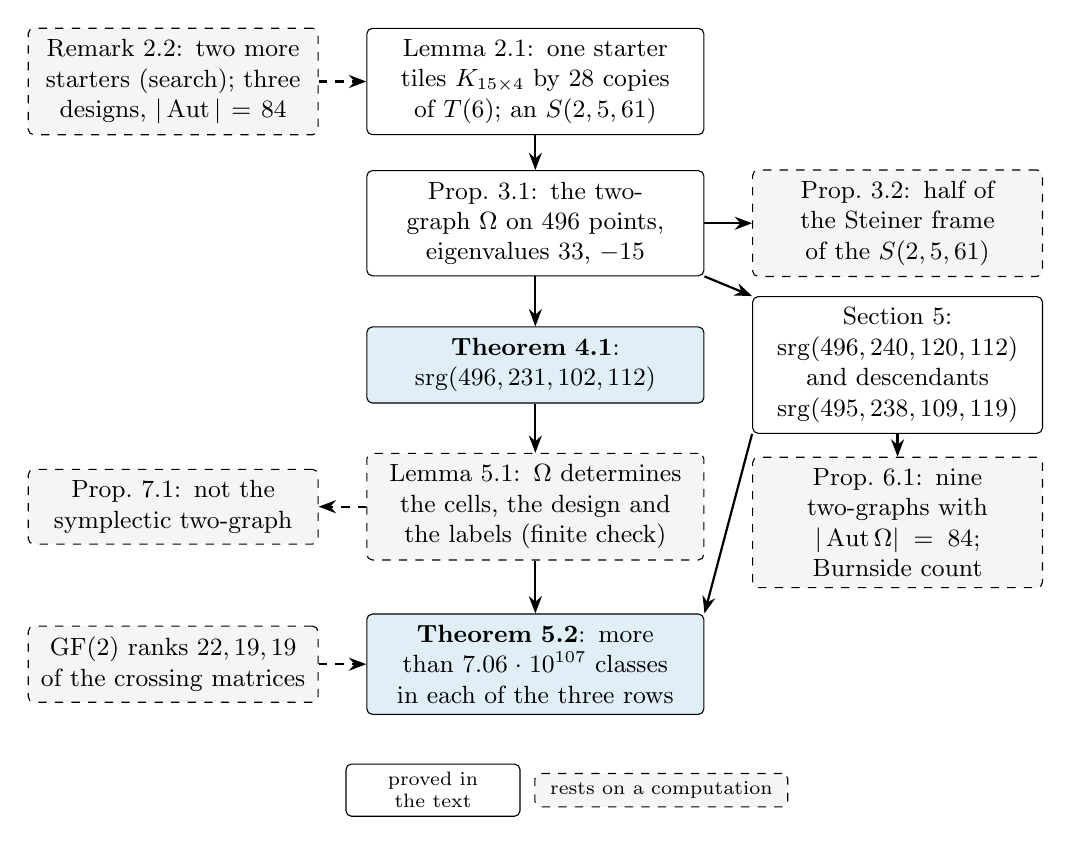
\begin{tikzpicture}[
  font=\small,
  box/.style={draw, rounded corners=2pt, align=center, text width=#1, inner sep=4pt, fill=white},
  box/.default=4.0cm,
  comp/.style={box=#1, dashed, fill=gray!8},
  comp/.default=3.4cm,
  arr/.style={-{Stealth[length=2.2mm]}, thick}]
% main column
\node[box] (til) at (0,0) {Lemma 2.1: one starter tiles $K_{15\times4}$ by $28$ copies of $T(6)$; an $S(2,5,61)$};
\node[box] (etf) at (0,-1.8) {Prop.~3.1: the two-graph $\Omega$ on $496$ points, eigenvalues $33$, $-15$};
\node[box, fill=pA!12] (thm) at (0,-3.6) {\textbf{Theorem 4.1}: $\srg(496,231,102,112)$};
\node[comp=4.0cm] (rec) at (0,-5.4) {Lemma 5.1: $\Omega$ determines the cells, the design and the labels (finite check)};
\node[box, fill=pA!12] (cnt) at (0,-7.4) {\textbf{Theorem 5.2}: more than $7.06\cdot10^{107}$ classes in each of the three rows};
% left column
\node[comp] (more) at (-4.6,0) {Remark 2.2: two more starters (search); three designs, $|\Aut|=84$};
\node[comp] (sp) at (-4.6,-5.4) {Prop.~7.1: not the symplectic two-graph};
\node[comp] (rk) at (-4.6,-7.4) {GF$(2)$ ranks $22,19,19$ of the crossing matrices};
% right column
\node[comp] (half) at (4.6,-1.8) {Prop.~3.2: half of the Steiner frame of the $S(2,5,61)$};
\node[box=3.4cm] (oth) at (4.6,-3.6) {Section 5: $\srg(496,240,120,112)$ and descendants $\srg(495,238,109,119)$};
\node[comp] (sym) at (4.6,-5.6) {Prop.~6.1: nine two-graphs with $|\Aut\Omega|=84$; Burnside count};
% arrows
\draw[arr] (til) -- (etf); \draw[arr] (etf) -- (thm); \draw[arr] (thm) -- (rec); \draw[arr] (rec) -- (cnt);
\draw[arr, dashed] (more) -- (til);
\draw[arr] (etf) -- (half);
\draw[arr] (etf.south east) -- (oth.north west);
\draw[arr] (oth) -- (sym);
\draw[arr] (oth.south west) -- (cnt.north east);
\draw[arr, dashed] (rec) -- (sp);
\draw[arr, dashed] (rk) -- (cnt);
% legend
\node[box=2.0cm, inner sep=3pt, font=\scriptsize] (lg1) at (-1.3,-9.0) {proved in the text};
\node[comp=3.0cm, inner sep=3pt, font=\scriptsize] at (1.6,-9.0) {rests on a computation};
\end{tikzpicture}
}
\caption{How the results depend on each other. Solid boxes are proved in the text, and dashed boxes rest on a computation listed in Section~\ref{sec:data}.}
\label{fig:flow}
\end{figure}

\subsection*{Use of AI}
AI assistants were used for the search and verification programs and for a first draft of the text. GPT~6.2 Astra proposed the initial constructions. Claude Opus~5.5 audited and verified them and helped draft the first version of this note. The author has verified and finalized all results and text.

\begin{thebibliography}{9}
\bibitem{BrTab} A.~E.~Brouwer, Parameters of strongly regular graphs, \url{https://aeb.win.tue.nl/graphs/srg/srgtab.html}.
\bibitem{FJMPW18} M.~Fickus, J.~Jasper, D.~G.~Mixon, J.~D.~Peterson and C.~E.~Watson, Equiangular tight frames with centroidal symmetry, \emph{Appl. Comput. Harmon. Anal.} 44 (2018) 476--496.
\bibitem{FMT12} M.~Fickus, D.~G.~Mixon and J.~C.~Tremain, Steiner equiangular tight frames, \emph{Linear Algebra Appl.} 436 (2012) 1014--1027.
\bibitem{Krc} V.~Kr\v{c}adinac, Steiner $2$-designs $S(2,6,76)$, \url{https://web.math.pmf.unizg.hr/~krcko/results/steiner/2-76-6-1.des}.
\bibitem{P400} D.~Plummer, Strongly regular graphs with parameters $(400,168,68,72)$, note, 2026.
\bibitem{P442} D.~Plummer, Strongly regular graphs with parameters $(442,231,120,121)$ from Mathon's conference two-graph, \url{https://github.com/dylan-plummer/srg442}.
\bibitem{Sei76} J.~J.~Seidel, A survey of two-graphs, in \emph{Colloquio Internazionale sulle Teorie Combinatorie (Roma, 1973)}, Tomo I, Accad. Naz. Lincei, Rome, 1976, 481--511.
\bibitem{Tay77} D.~E.~Taylor, Regular $2$-graphs, \emph{Proc. London Math. Soc. (3)} 35 (1977) 257--274.
\end{thebibliography}

\end{document}
